\section{Сравщнительная оценка погрешностей}

Сравним результаты, полученные аналитическим методом и алогоритмом Баруна--Робинсон.
На таблице~\ref{tab:tab2} представлены смешанные стратегии обоих игроков, цены игр,
абсолютная и относительная погрешности.

\begin{table}[h]
    \centering
    \caption{Сводная таблица сравнительной оценки погрешностей}
    \begin{tabularx}{\textwidth}{|X|c|c|c|c|c|c|c|} \hline
        & Цена игры & $a_1$ & $a_2$ & $a_3$ & $b_1$ & $b_2$ & $b_3$ \\ \hline
        Аналитический (матричный) метод & 12.992 & 0.530 & 0.114 & 0.356 & 0.341 & 0.129 & 0.530 \\ \hline
        Численный метод Брауна-Робинсон & 13.009 & 19.000 & 4.000 & 12.667 & 11.667 & 6.667 & 17.333 \\ \hline
        Абсолютная погрешность, $\Delta$ & 0.017 & 18.470 & 3.886 & 12.311 & 11.326 & 6.538 & 16.803 \\ \hline
        Относительная погрешность, \% & 0.13 & 3484.9 & 3410.5 & 3458.1 & 3321.1 & 5069.8 & 3171.3 \\ \hline
    \end{tabularx}
    \label{tab:tab2}
\end{table}

Абсолютная погрешность считается по формуле~\ref{f4}:

\begin{equation}\label{f4}
  \Delta = \left| X_{\text{численный}} - X_{\text{аналитический}} \right|
\end{equation}

Относительная погрешность считается по формуле~\ref{f5}:

\begin{equation}\label{f5}
\varepsilon = \frac{\Delta}{X_{\text{аналитический}}} \times 100\%
\end{equation}

Графики сходимости приближенных значений цен игры и оценки погрешности приведены на рисуках \ref{fig:fig4} и \ref{fig:fig5} соответственно.

\begin{figure}
  \centering
  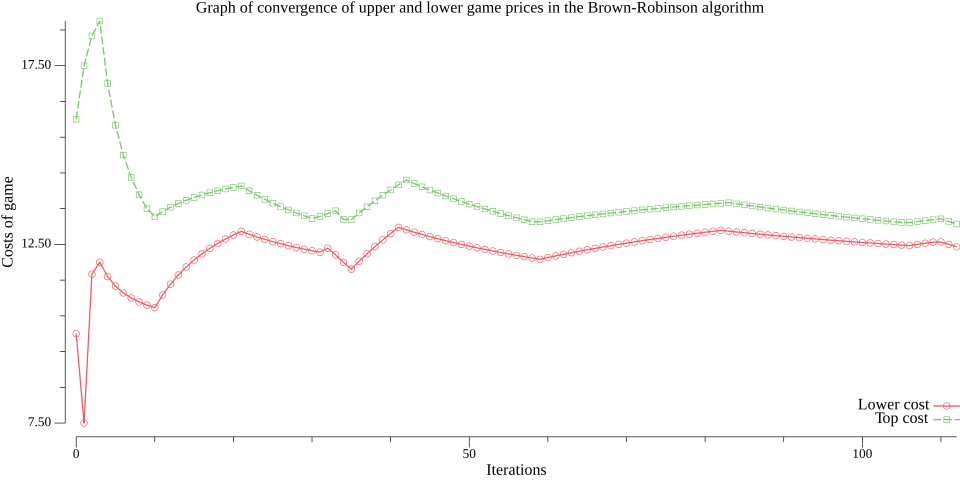
\includegraphics[scale=0.5]{../../artifacts/lw1/costs.png}
  \caption{График сходимости верхней и нижней цен игры в алгоритме Брауна--Робинсон}
  \label{fig:fig4}
\end{figure}

\begin{figure}
  \centering
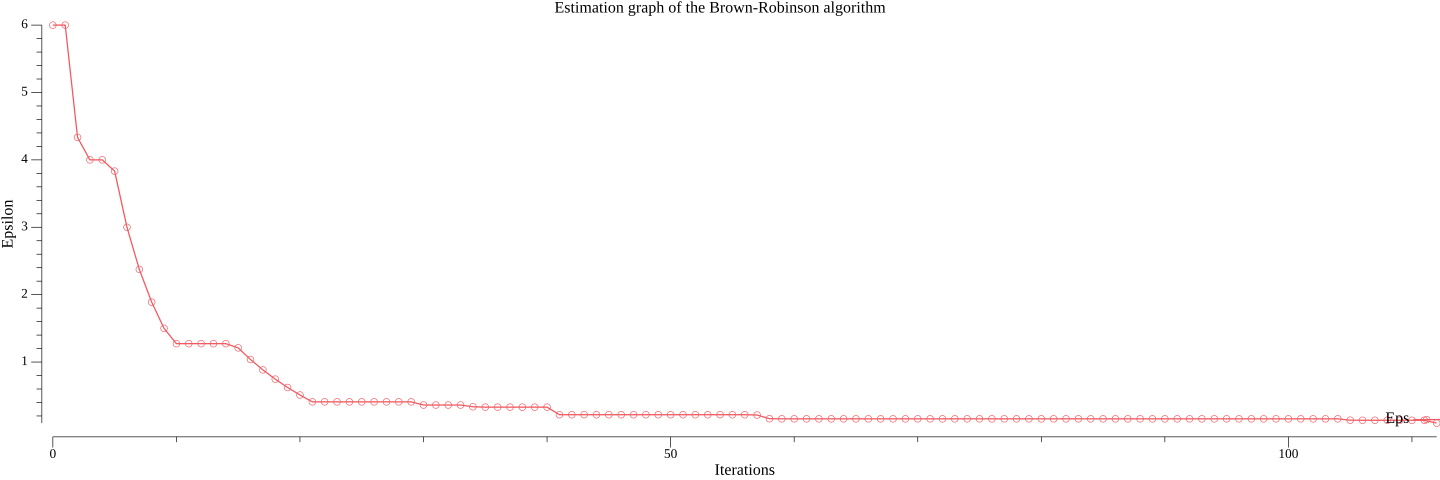
\includegraphics[scale=0.5]{../../artifacts/lw1/estimation.png}
  \caption{График оценки погрешности алгоритма Брауна--Робинсон}
  \label{fig:fig5}
\end{figure}
